%% introduction.tex
%%

%% ==============================
\chapter{Introduction}
\label{ch:Introduction}
%% ==============================
	The neutrino was not discovered in the conventional meaning but postulated by Wolfgang Pauli, then under the name neutron, as a explanation for the spectrum of the beta decay showing a continous energy distribution which did not concur with the idea of a two body decay \cite{fermi}. 
	\begin{equation}
		\ce{p -> n + e^-}
	\end{equation}
	Coservation laws of energy, momentum and angular momentum were violated.
	The neutrino solved this problem by being a carrier of different kinetic energies thus allowing for a continuous spectrum.
	\begin{equation}
		\ce{p -> n + e^- + \bar\nu_e}
	\end{equation}
	To be compliant with the laws of conversation, the new particle needed to be of spin 1/2 and chargeless.
	The first experimental evindence for this particle was then given by Cowan and Reines \cite{neutrinoEvidence} who observed the reaction of electron-anti-neutrinos and free protons in the large neutrino flux of a nearby nuclear reactor.
	\begin{equation}
		\ce{\bar\nu_e + p -> e^+ + n}
	\end{equation}
	They then looked for two events: a pair of \SI{511}{\kilo\electronvolt} photons from electron-positron anihilation as well as the $\gamma$ from neutron capture some \SI{}{\micro\second} afterwards.
	Following the electron neutrino, both other known neutrino gernations have been attested for in various experiments, the first ones to find evidence for $\nu_\mu$ and $\nu_\tau$ were to be Danby and Gaillard \cite{muNeutrino} and the DONUT experiment \cite{tauNeutrino} respectively.
	
	\section{Neutrino sources}
	\label{ch:Introduction:sec:neutrinoSources}
	\begin{itemize}
		\item Primordial neutrinos\\
		Lingering around since the ``Big Bang'', neutrinos with rather low, thermal energies form a cosmic neutrino background. 
		
		\item Solar Neutrinos
		
		\item Reactor neutrinos
	\end{itemize}

	
	
    \section{Neutrinos in the standard model}
    \label{ch:Introduction:sec:Neutrinos in the standard model}
    During the second part of the 20th century, a model stating 16 particles has been developed to describe a huge portion of known phenomena, the standard model. It contains six isquarks, six leptons (both made up of three particle generations) and four types of Gauge Bosons. The latter are carriers of the standard models interactions of the former particles, meaning all interactions of matter are based on the exchange of one or more of the Gauge Bosons. 
    For our universe, gravity, the graviton generated force, plays a major role for formation and stability af almost all larger structures. In particle physics however, it can mostly be neglected. Here, only the strong and weak as well as the electromagnetic interaction make for noticable contributions to phenomena observed. That is why, in the standard model, gravity as well as its carrier, the graviton, are disregarded.
    \begin{figure}
    	\centering
    	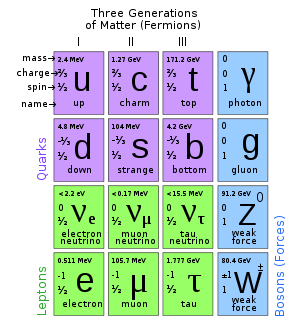
\includegraphics[width = 0.6\textwidth]{graphics/standardModel/particles.png}
    	\caption[standard model particles]{Particles stated in the standard model. On the upper left quarks, on the lower left leptonic particles. The very right row contains the bosonic force particles. Note the absence of the graviton.\cite{particlesSM}}
    	\label{fig:standardModel:particles}
    \end{figure}
	
    Most of what we can observe with our bare eyes or in basic experiments is attributable to the electromagnetic force or gravity, however, strong and weak interaction do play a major role when it comes to high energy physics. Here, the limited reach of the two is overcome by small distances between interacting particles. In case of the neutrino, detection and by that the study of its characteristics is even more difficult as it interacts only gravitationally and weakly. Now, as mentioned before, gravity is indeed long range, but very weak in force. And although weak intraction is a lot stronger compared to gravity, it is still weak compared to both electromagnetic and strong interactions. That is why the neutrino is considered elusive, detection efficiencies are low and only large scale detectors are able to detect statistically relevant amounts of neutrinos.
    One method used quite frequently is the Cherenkov radiation emitted while travelling through matter at speeds above the speed of light. This light, comparable to the supersonic cones planes cause in air, can be detected by standard photomiltiplier tubes. The problem is that, as mentioned above, the volumes to be able to make dependable statements on directions and energies need to be large. This is why most experiments make use of ``natural'' detectors such as water \todo{cite MARE+ICE Cube} or even ice.
    Other approaches are to catch neutrinos in reactions where those are required such as inverse beta decays:
    \begin{equation}
		\ce{\bar\nu_e + p -> e^+ + n}
    \end{equation}
   
    
    In the standard model, neutrinos are considered massless. 
    Many experiments though have shown that the weightless neutrino is a wrong assumption. Most of these were experiments prooving neutrino oscillatinos with both reactor neutrinos and solar neutrinos such as Kamiokande\cite{PhysRevLett.110.181802} or SNO \cite{SNOOscillations} \todo{add experiments}.
    Important for those experiments is the known source location making baseline analysis possible.
    
    Up till now, only the differences of the squared masses are known. This leads to different relations depending on how masses are distributed between the flavours, see figure \ref{fig:massSchemes}, and how large they are absolutely, see figure \ref{fig:massHierarchy}. This problem is solved by the knowledge of one of the masses. KATRIN is on the verge of finding the $\nu_e$'s mass. Two mass schemes are possible: the normal and the inverted one. Normal means that the smallest number also describes the smallest mass state, i.e. $m_{\nu_1} < m_{\nu_2} < m_{\nu_3}$. In the inverted scheme, the squared mass difference of eigenstates two and three is not directed upwards, but pushes the $m_{\nu_3}$ mass below the two others.
    
    \begin{figure}
    \centering
    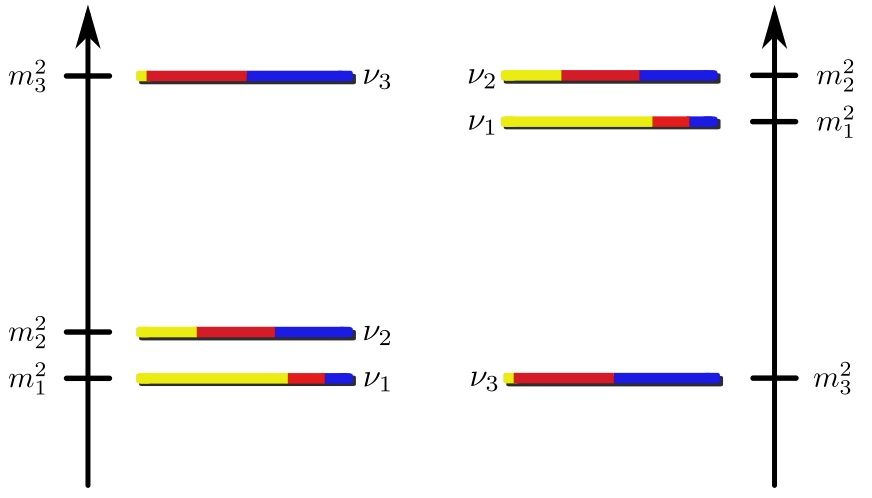
\includegraphics[width=0.5\textwidth]{graphics/standardModel/massHierarchy.jpg}
    	 \caption[Neutrino mass hierarchy]{The possible mass hierarchies for neutrinos. Left, the normal scheme with $m_{\nu_1} < m_{\nu_2} < m_{\nu_3}$, on the right the normal scheme where $m_{\nu_1} < m_{\nu_2}$ is still true, though both $m_{\nu_3} < m_{\nu_1}$ and $m_{\nu_3} < m_{\nu_2}$ }. The coloured bars represent the matrix elements for each flavour, i.e. the probabilities, or composition of each flavour eigenstate.
    	\label{fig:massSchemes}
    \end{figure}
    \begin{figure}
    \centering
    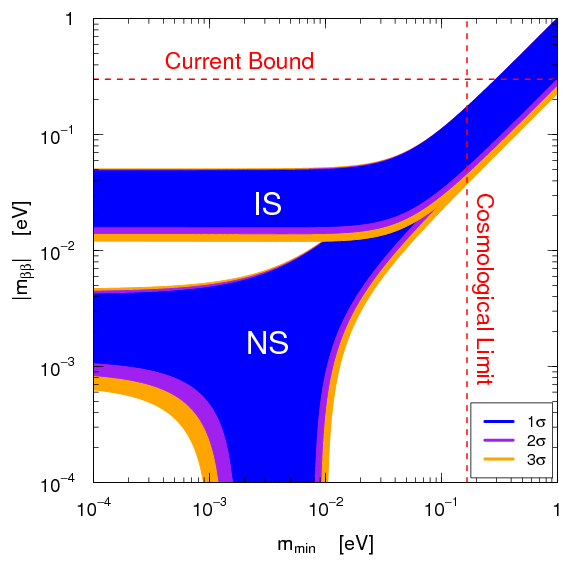
\includegraphics[width = 0.5 \textwidth]{graphics/standardModel/massSchemes.png}
	\caption[Effective neutrino mass]{The possible effective masses for neutrinos depending on the lightest neutrino mass $m_{min}$ shown on the x-axis. Normal and inverted scheme are marked NS and IS. The current bound from $0\nu\beta\beta$ decay is displayed as well as cosmological limitations. }
    	\label{fig:massHierarchy}
    \end{figure}

    
    \subsection{Neutrino Oscillations}
    \label{ch:Introduction:sec:Massive neutrino:subsec:neutrino Oscillations}
      If the neutrinos were without mass, its mass eigenstates would equal its flavour eigenstates:
      
    \begin{equation}
% 	\begin{array}{ccc}
%       	|\nu_e>		& = & |\nu_1>\\
%       	|\nu_\mu>	& = & |\nu_2>\\
%       	|\nu_\tau>	& = & |\nu_3>\\
%     	 \end{array}
    \end{equation}
    First doubts concerning this asumptions occured as inconsistencies between the measured and the calculated solar $\nu$-flux occured. As the count on $\nu_e$ was too low, the theory of neutrino oscillations emerged, stating that a mixture of flavours was possible as the flavours were made up of all three of the mass eigenstates. The mixture is described by the so called Pontecorvo-Maki-Nakagawa-Sakata matrix:
        \begin{equation}
        \left(
        \begin{array}{c}
	  |\nu_e>\\
	  |\nu_\mu>\\
	  |\nu_\tau>\\
        \end{array}
        \right)
	 = \left(
	\begin{array}{ccc}
      	U^*_{e,1} & U^*_{e,2} & U^*_{e,3}\\
      	U^*_{\mu,1} & U^*_{\mu,2} & U^*_{\mu,3}\\
      	U^*_{\tau,1} & U^*_{\tau,2} & U^*_{\tau,3}\\
      	\end{array}
	\right)
	\left(
	\begin{array}{c}
      	|\nu_1>\\
      	|\nu_2>\\
      	|\nu_3>\\
    	 \end{array}
    	 \right)
    \end{equation}
    In this equation, the matrix U can be parametrized through a combination of three rotation matrices and a complex phase factor $\delta_D$ as well as two complex majorana phases $\delta_M$
    
    \begin{equation}
	\centering
	\begin{split}
     U = \left(
	\begin{array}{ccc}
      	1 & 0 & 0\\
      	0 & c_{23} & s_{23}\\
      	0 & -s_{23} & c_{23}\\
   	\end{array}
	\right)
	\left(
	\begin{array}{ccc}
      	c_{13} & 0 & s_{13}e^{-i\delta_D}\\
      	0 & 1 & 0\\
      	-s_{13}e^{-i\delta_D} & 0 & c_{13}\\
      	\end{array}
	\right)\cdot\\
	\cdot\left(
	\begin{array}{ccc}
      	c_{12} & s_{12} & 0\\
      	-s_{12} & c_{12} & 0\\
      	0 & 0 & 1\\
      	\end{array}
	\right)
		\left(
	\begin{array}{ccc}
      	e^{i\delta_{M1}} & 0 & 0\\
      	0 & e^{i\delta_{M2}} & 0\\
      	0 & 0 & 1\\
      	\end{array}
	\right)
	\end{split}
    \end{equation}
    where $c_{ij}=\cos{\theta_{ij}}$ and $s_{ij}=\sin{\theta_{ij}}$.\\
	Now the pure eigenstate of a neutrino for t=0 can be described by three matrix elements and the corresponding mass eigenstates.
	\begin{equation}
		\left|\nu(t=0)\right> = \left|\nu_\alpha\right> = U^*_{\alpha1} \left|\nu_1\right> + U^*_{\alpha2} \left|\nu_2\right> + U^*_{\alpha3} \left|\nu_3\right> 
	\end{equation}
	The time evolution of this state now reveals the oscillations of the neutrino from flavour to flavour, as the time evoluted states are not flavour eigenstate for every point in time.
	\begin{equation}
		\left|\nu_\alpha(t>0)\right> = U^*_{\alpha1} e^{-iE_{\alpha1}t}\left|\nu_1\right> + U^*_{\alpha2} e^{-iE_{\alpha2}t}\left|\nu_2\right> + U^*_{\alpha3}e^{-iE_{\alpha3}t} \left|\nu_3\right> \neq \left|\nu_\alpha\right> 
	\end{equation}
	
	\begin{equation}
		\left|\nu_\alpha(t)\right> = \sum_{k = 1,2,3} U_{\alpha k}\exp\left(-iE_k t\right)\left|\nu_k\right>
	\end{equation}
	for every state $\left|\nu_\alpha\right>$ where the mass eigenstates have in turn been expressed as a mixture of flavour eigenstates.

	The probability for a flavour $\left|\nu_i\right>$ to exist after a certain period of time is given by the multiplication with the 
	
    
    
    \subsection{Direct measurement of neutrino mass}
    \label{ch:Introduction:sec:Massive neutrino:subsec:direct Neutrino Mass measurement}
    Direct measurements of the neutrino mass require a reaction known to include neutrinos in its equation. There are both spectrometric and calorimetric approaches. While the scale of spectrometers is getting bigger and bigger, calorimetric approaches seem to be a reasonable alternative, although the slow detector response - the detector material itself is decaying - requires for large arrays of detectors leading to extensive space requirements as well at some point. The luminosity of spectrometer experiments though is unachieved by any other. That is why the KATRIN collaboration is working on a setup to measure electrons from Tritium decay to determine the neutrino mass. 
     
    \subsection{Indirect measurement of neutrino mass}
    \label{ch:Introduction:sec:Massive neutrino:subsec:indirect Neutrino Mass measurement}
    Another approach is using indirect ways of finding the neutrino mass. One possibility here is to search for neutrinoless double beta decay, $0\nu\beta\beta$, which can exist only if the neutrino is its own anti-particle, a so called majorana neutrino. Then, if two nuclei beta decay, the neutrino from one vertex can be absorbed in the second as an anti-neutrino - or vice versa. The decay would then not emit any neutrino and the rate would be dependant on the effective Majorana neutrino mass square'' \cite{currentNeutrinoSearches}:
    \begin{equation}
    	\Gamma_{0\nu\beta\beta} \propto \left| \sum{U_{ei}^2m\left(\nu_i\right)}\right|^2
    \end{equation}

    
    \section{Cosmic muons and their interaction with matter from the viewpoint of KATRIN}
    \label{ch:introduction:sec:Cosmic Air Showers}
    When high energy particles hit the upper parts of the atmosphere, a cascade of particles generated from the interaction with atmospheric molecules and atoms follows. Most primary particles are nucleons, most of which again are free protons, i.e. Hydrogen ions. Helium nucleons' fluxes are already about a order of magnitude below that, higher mass number nuclei show even lower rates\cite{highEnergyCosmicRays}. 
    \begin{figure}
	\begin{minipage}[d]{0.49 \textwidth}
		  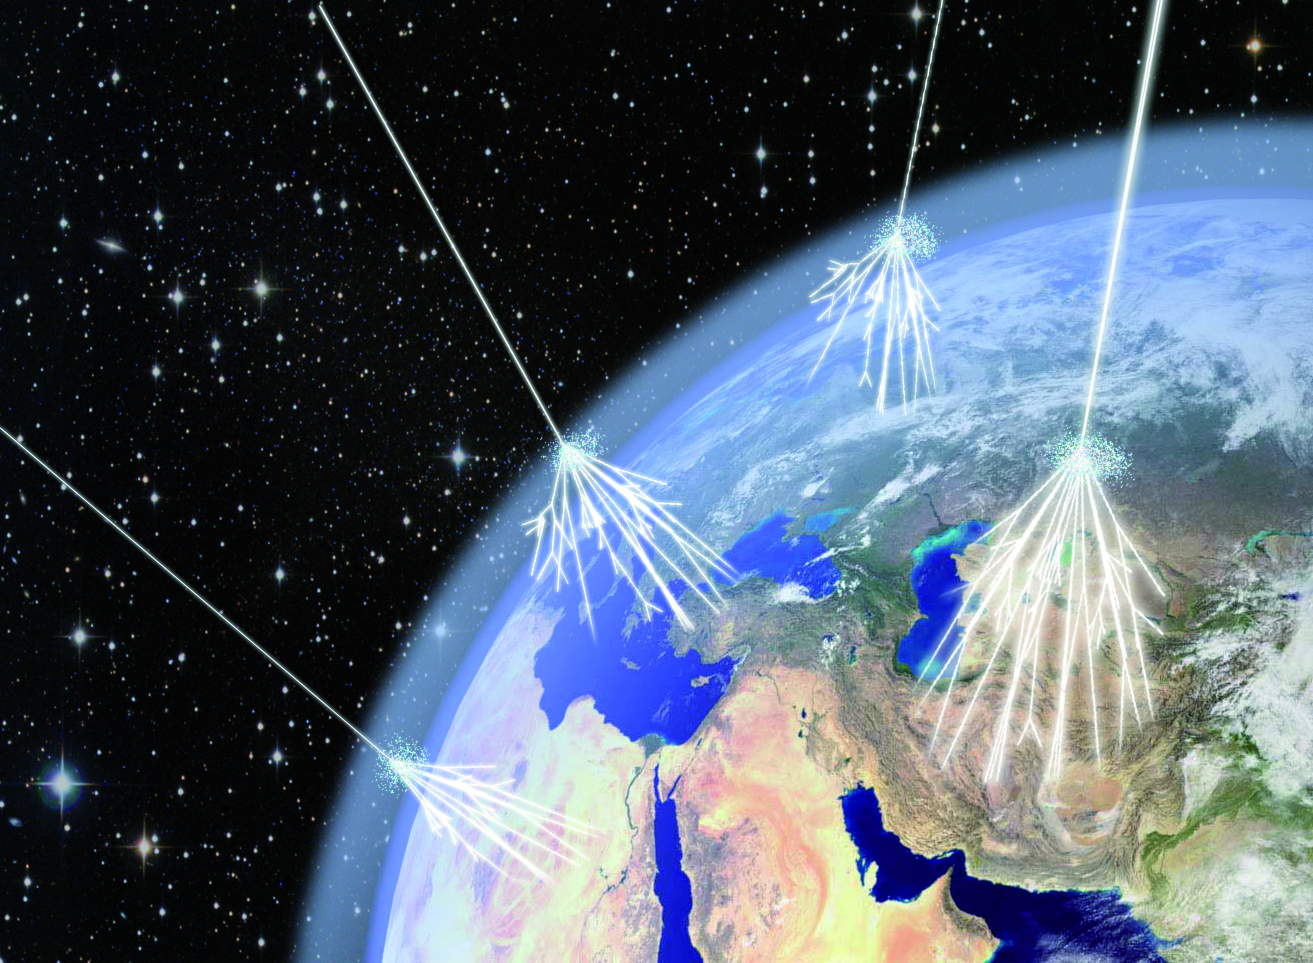
\includegraphics[width=\textwidth]{graphics/cosmicRays/cosmicRays.jpg}
	\end{minipage}
	\begin{minipage}[d]{0.49 \textwidth}
		  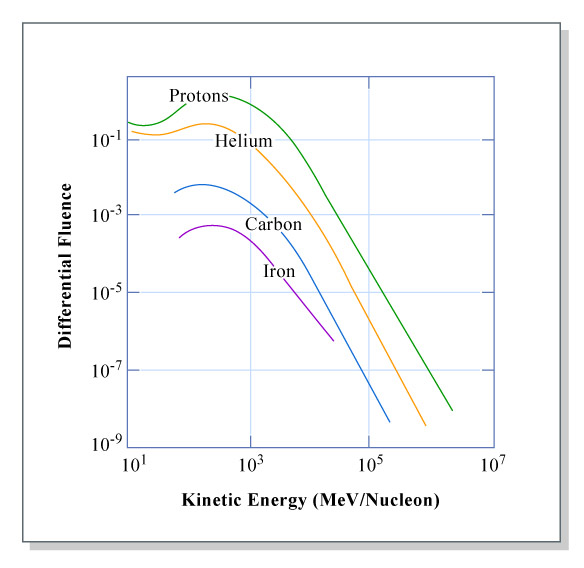
\includegraphics[width=\textwidth]{graphics/cosmicRays/energySpectrum.jpg}
	\end{minipage}
	\caption[Cosmic ray composition]{On the left, an artistic impression of various cosmic rays hitting the atmosphere \cite{airShower}. On the right, the measured composition for cosmic nuclei is shown: on top, the lightest particle, the proton. further down, all with orders of magnitude smaller rates, heavier ions.}
    \end{figure}
    \todo{insert right side graphic from TODOR}
    By different interactions, secondary partcles are created. Any particle satisfying the inequation \begin{equation}
      E_{sec,kin} + m_{sec} c^2 < E_{prim,kin} + m_{prim}
    \end{equation}
    can be created. Mostly pions at first, those cascade further. Often through intermediate photons, muons emerge. These travel towards the earths surface mostly close to the speed of light due to their small masses though high energies. Even at these high speeds, the muons' average decay time of around \SI{2.2}{\micro\second} \cite{muonLifetime} is too small for many muons to reach the earth's surface from our reference frame's point of view. In the most common production height of \SI{2}{\kilo\meter} \cite{muonProductionHeight}, the non relativistic time of flight for a \SI{90}{\percent} speed of light particle would be
    \begin{equation}
	t_{class} = \SI{2}{\kilo\meter} / 0.9\cdot c = 
    \end{equation}
    meaning only time dilation from special relativity makes the muon flux as large as ist is:
    \begin{equation}
    	t_{rel} = t_{class} / \sqrt{1-0.9^2}
    \end{equation}
    which, from our reference frame, prolongs the lifetime by a factor of around 5, being already enough to reach the surface from heights of \SI{3}{\kilo\meter}. Most muons have even higher energies, making it possible for them to reach surface from greater heigts and under non perpendicular angles towards it.
    For KATRIN, this poses a problem. A smaller flux would be advantageous, as muons may, through different kinds of interaction, cause emission of electrons from the spectrometer vessels surface. Shielding against muons is difficult as it requires thick layers of dense matter due to the muons high energies and the low deposition in matter in relations to those. 
    

